\documentclass{article}

%-------------------------%
% PREAMBUŁA --------------%
%-------------------------%
\usepackage[utf8]{inputenc}
\usepackage[OT4]{polski}
\usepackage{caption}
\usepackage{amsmath}
\usepackage{tikz}
\usepackage{subcaption}
\usepackage{tabularx}
\usepackage{caption}
\usepackage{array}
\usepackage{hyperref}
\usepackage{graphicx}
\usepackage{fancyhdr}
\usepackage[justification=centering]{caption}
\usepackage[margin=60pt]{geometry}
\usepackage{longtable}



%\usepackage[T1]{fontenc}
%\usepackage{amsthm}
%\theoremstyle{plain}
%\usepackage{enumitem}
%\captionsetup[table]{skip=-4pt}
%\usepackage{tabulary}
%\usepackage{sidecap}
%\usepackage{gensymb}
%\usepackage{wrapfig}
%\usepackage{lastpage}
%\usepackage{gensymb}
%\usepackage{lipsum}
%\pagestyle{fancy}


\newlength{\RoundedBoxWidth}
\newsavebox{\GrayRoundedBox}
\newenvironment{GrayBox}[1][\dimexpr\textwidth-4.5ex]%
   {\setlength{\RoundedBoxWidth}{\dimexpr#1}
    \begin{lrbox}{\GrayRoundedBox}
       \begin{minipage}{\RoundedBoxWidth}}%
   {   \end{minipage}
    \end{lrbox}
    \begin{center}
    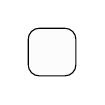
\begin{tikzpicture}%
       \draw node[draw=black,fill=black!1,rounded corners,%
             inner sep=2ex,text width=\RoundedBoxWidth]%
             {\usebox{\GrayRoundedBox}};
    \end{tikzpicture}
    \end{center}}

%------- Typy kolumn do ustawiania szerokości ------- %
\newcolumntype{L}[1]{>{\raggedright\let\newline\\\arraybackslash\hspace{0pt}}m{#1}}
\newcolumntype{C}[1]{>{\centering\let\newline\\\arraybackslash\hspace{0pt}}m{#1}}
\newcolumntype{R}[1]{>{\raggedleft\let\newline\\\arraybackslash\hspace{0pt}}m{#1}}








\begin{document}

%-------------------------%
%Tabela nagłówkowa -------%
%-------------------------%

\begin{table}[h]
\begin{tabular}{|l|l|l|l|l|l|}
\hline
\begin{tabular}[c]{@{}l@{}}
Wydział:\\ WFiIS\end{tabular} &
\multicolumn{2}{l|}{\begin{tabular}[c]{@{}l@{}}
Imię i nazwisko:\\ 1. Axel Zuziak\\ 2. Marcin Węglarz \end{tabular}} 
& Rok \textbf{II}         
& Grupa \textbf{B}          
& Zespół \textbf{03}      \\ \hline
\textbf{\begin{tabular}[c]{@{}l@{}}
LABOLATORIUM\\ TECHNIK \\ JĄDROWYCH\end{tabular}} &
\multicolumn{4}{l|}{ Temat:\textbf{ Statystyczny charakter rozpadów promieniotwórczych.}
	 }                                                                                                                       & \multicolumn{1}{c|}{\begin{tabular}[c]{@{}c@{}}
Nr ćwiczenia\\ \textbf{1+9}
\end{tabular}} \\ \hline
\begin{tabular}[c]{@{}c@{}}
Data wykonania:\\ 04.03.2015
\end{tabular} &
\begin{tabular}[c]{@{}c@{}}
 Data oddania:\\ 18.03.2015
\end{tabular} &
\begin{tabular}[c]{@{}c@{}}
Zwrot do poprawy: \\ 
\end{tabular}                                 
& 
\begin{tabular}[c]{@{}c@{}}
Data oddania: \\ 
\end{tabular}&
\begin{tabular}[c]{@{}c@{}}
Data zaliczenia:\\
\end{tabular}& 
\begin{tabular}[c]{@{}c@{}}
OCENA:\\
\end{tabular}       
\\ & & & & & \\ \hline
\end{tabular}
\end{table}
%-----Koniec tabeli------

%%%%%%%%%%%% Wstęp %%%%%%%%%%%%
\section{Cel ćwiczenia}
Celem ćwiczenia jest wyznaczenie zawartości procentowej wodoru w badanej próbce metodą neutronową. Przybliżenie zagadnienia detekcji neutronów oraz ich oddziaływania z materią.
\section{Wstęp teoretyczny}
Ideą ćwiczenia jest wykorzystanie faktu, że wodór jest wyjątkowo dobrym spowalniaczem neutronów (neutrony tracą przy zderzeniu centralnym prawie 100\% swojej energii kinetycznej), ze względu na zbliżone masy atomu wodoru oraz neutronu. Jeżeli na próbke będą padały jedynie neutrony prędkie to strumień neutronów termicznych po przejściu przez próbkę będzie proporcjonalny do gęstości atomów wodoru w badanym materiale. \\

Jako źródło neutronów wykorzystuję się źródło Pu-Be, gdzie pluton jest emiterem cząstek alfa, 
które następnie ulegają reakcji z jądrami berylu, który ma niską energię separacji neutronu.\\
\[^9_4\text{Be }(\alpha,n)\ ^{12}_6\text{C}\]
Neutrony powstałe w powyższej reakcji mają różne prędkości, natomiast w doświadczeniu potrzebny jest jedynie strumień neutronów prędkich. W tym celu pomiędzy źródłem a badaną próbką umieszcza się osłonę kadmową. Kadm wykazuję szczególnie duży przekrój czynny na absorpcję neutronów termicznych i przekrój ten gwałtownie maleje dla wyższych energii, dzięki czemu pełni ona rolę filtra przepuszczającego jedynie neutrony o większej energii.\\\\
Kolejnym punktem na drodze strumienia neutronów jest już badana próbka. Jak wspomniano powyżej wodór ze względu na praktycznie identyczną masę z masą neutronu bardzo wydajnie je spowalnia. W praktyce większość neutronów spowolnionych przez próbkę jest wynikiem ich oddziaływania z jądrami wodoru, dzięki czemu możemy szukać korelacji pomiędzy ilością zliczeń neutronów termicznych w detektorze, a gęstościa wodoru w badanej próbce (ponieważ przekrój czynny na oddziaływanie neutronów z jądrami wodoru w głównej mierze zależy od  gęstości H). \\\\
Przed przystąpieniem do wyznaczania nieznanej zawartości wodoru należy wyznaczyć prostą korelacji częstości zliczeń od znanej zawartości wodoru w próbkach wzorcowych. W tym celu do punktów pochodzących z próbek wzorcowych wystarczy dopasować prostą na przykład metodą najmniejszych kwadratów.\\\\
Po przejściu przez próbkę neutrony wpadają do detektora. W doświadczeniu jako detektora użyto licznika proporcjonalnego z dodatkiem gazowego BF$_3$. Detekcja neutronów sprawia pewne problemy, ponieważ nie jonizują one materii. Obejściem tego problemu jest właśnie dodatek trójfluorku boru. Bor posiada duży przekrój czynny na absorpcję neutronów termicznych (neutrony termiczne są też lepiej absorpowane ze względu na regułę $1/v$, mówiącej że przekrój czynny na oddziaływanie z neutronami jest odwrotnie proporcjonalny do ich prędkości). \\\\
W detektorze zachodzi reakcja przedstawiona na Rysunku \ref{rozpad_boru}. Jak widać z powyższego rysunku reakcja ma dwa kanały rozpadu, dzięki czemu obserwujemy dwa piki przesunięte względem siebie o około 0,48 MeV. Cząstki alfa oraz jądra litu jonizują dalej materię co prowadzi do wytworzenia impulsu elektrycznego, który następnie jest wzmacniany i przy pomocy analizatora oraz przelicznika zliczany.

\begin{figure}[h!]
	\centering
	\includegraphics[width=0.8\textwidth]{images/rozpad_boru.png}
	\caption{Reakcja rozpadu boru pod wpływem absorpcji neutronu termicznego.\cite{DzK}}
	\label{rozpad_boru}
\end{figure}




\section{Aparatura i wykonanie ćwiczenia}
\begin{itemize}
	\item \textbf{Neutronowy miernik wodoru}
	\item \textbf{Wzmacniacz impulsowy}
	\item \textbf{Zasilacz wysokiego napięcia}
	\item \textbf{Analizator amplitudy}
	\item \textbf{Przelicznik}
\end{itemize}

Ćwiczenie rozpoczęto od zapoznania się z aparaturą pomiarową. Przed przystąpieniem do wykonywania pomiarów zmierzono wszystkie wymiary geometryczne zarówno próbek wzorcowych: $W1,W2,...W7$ jak i tych, dla których wyznaczano gęstość wodoru: $P1,P2,...P7$. Zanotowano wagi poszczególnych próbek. Następnie rozpoczęto pomiary częstości detekcji neutronów termicznych dla siedmiu próbek wzorcowych, ustawiając czas detekcji na 100s. Wyniki przedstawiono w tabeli \ref{tabela_czestosci}. \\
Po zbadaniu próbek wzorcowych analogicznie zmierzono siedem próbek badanych. Wyniki przedstawiono w tabeli \ref{tabela_czestosci} oraz na wykresie (Rysunek \ref{krzywa}).

\section{Wyniki pomiarów i obliczenia.}

\subsection{Wyznaczenie objętości i gęstości badanych próbek.}
Przy pomocy linijki zmierzono wymiary geometryczne badanych próbek. Wyniki pomiarów i obliczeń przedstawiono w tabeli \ref{wynikiW}.

\begin{table}[h!]
\centering
\label{wynikiW}
\caption{Wymiary geometryczne próbek wzorcowych.}
\begin{tabular}{|C{2cm}|C{2cm}|C{2cm}|C{2cm}|}\hline
	Próbka & Waga [g] & Objętość [cm$^3$] & Zawartość $H$ [\%] \\ \hline
		W7	&	298,4	&	346,40	&	15,1 \\ \hline
		W6	&	436,25	&	361,28	&	8,89 \\ \hline
		W5	&	414,5	&	345,58	&	8,08 \\ \hline
		W4	&	478,44	&	338,70	&	6,42 \\ \hline
		W3	&	538,28	&	346,40	&	5,45 \\ \hline
		W2	&	434,46	&	337,72	&	2,05 \\ \hline
		W1	&	766,3	&	361,28	&	0 \\ \hline

\end{tabular}
\end{table}

\begin{table}[h!]
\centering
\label{wynikiP}
\caption{Wymiary geometryczne badanych próbek}
\begin{tabular}{|C{2cm}|C{2cm}|C{2cm}|C{2cm}|}\hline
	Próbka & Waga [g] & Objętość V [cm$^3$] & U(V) [cm$^3$] \\ \hline
		P1	&	181,31	&	331,89	&	10,14 \\ \hline
		P2	&	371,6	&	345,58	&	10,46  \\ \hline
		P3	&	511,34	&	345,58	&	10,46 \\ \hline
		P4	&	590,2	&	310,37	&	9,78 \\ \hline
		P5	&	593,58	&	338,70	&	10,30 \\ \hline
		P6	&	416,6	&	346,40	&	10,40 \\ \hline
		P7	&	439,47	&	361,28	&	10,67 \\ \hline

\end{tabular}

\end{table}

\begin{table}[h!]
	\centering
	\caption{Tabela zawierająca liczbę zliczeń w czasie 100s, a także odpowiednie wartości gęstości oraz stężenia wodoru w danej próbce.}
	\begin{tabular}{|c|c|c|c|c|c|}
		\hline
		Próbka & Liczba zliczeń $N$ & Gęstość $\rho _H$ & $u(\rho _H)$ & Stężenie $c$ [\%] & $u(c)$ [\%] \\\hline
		W7 & 65035 & 0.1300 & - & 15.10 & - \\\hline 
		W6 & 56688 & 0.1073 & - & 8.89 & - \\\hline 
		W5 & 52691 & 0.0969 & - & 8.08 & - \\\hline 
		W4 & 48084 & 0.0906 & - & 6.42 & - \\\hline 
		W3 & 44622 & 0.0846 & - & 5.45 & - \\\hline 
		W2 & 18598 & 0.0263 & - & 2.05 & - \\\hline 
		W1 & 11276 & 0.0000 & - & 0.00 & - \\\hline 
		 & & & & & \\\hline
		P1 & 20634 & 0.0259 & 0.0031 & 4.74 & 0.58 \\\hline 
		P2 & 55253 & 0.1064 & 0.0047 & 9.90 & 0.53 \\\hline 
		P3 & 15683 & 0.0144 & 0.0030 & 0.97 & 0.21 \\\hline 
		P4 & 14594 & 0.0119 & 0.0030 & 0.62 & 0.16 \\\hline 
		P5 & 15017 & 0.0129 & 0.0030 & 0.73 & 0.17 \\\hline 
		P6 & 52814 & 0.1007 & 0.0045 & 8.38 & 0.45 \\\hline 
		P7 & 56700 & 0.1098 & 0.0047 & 9.02 & 0.47 \\\hline 
		
		
	\end{tabular}
	\label{tabela_czestosci}
\end{table}



\newpage
\subsection{Cechowanie neutronowego miernika wodoru}
Do otrzymanych wyników dla próbek wzorcowych (tabela \ref{tabela_czestosci}) dopasowano prostą metodą regresji korzystając z programu Gnuplot:
\begin{equation}
	J = a_0 + a_1\rho_H
\end{equation}
 Otrzymano wartości:
 \begin{equation*}
 	a_1 = 43,0 \pm 1,5\cdot 10^4
 \end{equation*}
 \begin{equation*}
 	a_0 = 9500 \pm 1300
 \end{equation*}
Zatem otrzymana krzywa cechowania przyjmuje postać:
\begin{equation*}
	J = 430000\rho_H + 9500
\end{equation*}
Następnie przekształcono powyższe równanie do postaci\\
\[\rho _H = \frac{J-a_0}{a_1} = \frac{J-9500}{430000}
\]
po czy na podstawie tego równania oraz wyników częstości dla badanych próbek (tabela \ref{tabela_czestosci}) policzono gęstości wodoru. \\
Chcąc policzyć zawartość procentową wodoru pomnożono otrzymane gęstości przez objętość próbki, a następnie podzielono przez jej masę. Do wyznaczenia niepewności korzystano z prawa przenoszenia niepewności:
\[u(\rho _H) = \sqrt{ \Bigg[ \frac{-u(a_0)}{a_1} \Bigg]^2 + \Bigg[ \frac{-(J-a_0)}{a_1^2}u(a_1) \Bigg]^2 }
\]\\

\noindent
Obliczone wartości umieszczono w tabeli \ref{tabela_czestosci}.\\\\
Mając gęstość wodoru w badanej próbce oraz jej wymiary geometryczne i masę, możemy wyznaczyć zawartość 
procentową wodoru $c$ ze wzoru:
\begin{equation}
c = \frac{\rho _H V}{m}
\end{equation}
Natomiast niepewność z prawa przenoszenia niepewności pomiarowej:
\begin{equation}
u(c) = \sqrt{ \Big[ \frac{V}{m}u(\rho _H) \Big]^2 + \Big[ \frac{\rho _H}{m}u(V) \Big]^2}
\end{equation}\\\\\\

Jak widać z Rysunku \ref{krzywa}, częstość zliczeń jest skorelowana z zawartością wodoru, dzięki czemu metoda ta pozwala na wyznaczenie wilgotnośći materiału (należy pamiętać o odjęciu stałej gęstości wodoru dla danego materiału nie będącego składnikiem wody). Dodatkowo dokładniejsze pomiary wielkości próbki, a także większa ilość próbek wzorcowych mogą poprawić dokładność tej metody.




\begin{figure}[h!]
	\fontsize{6}{8}\selectfont % zmniejszam czcionke
	\centering
	\resizebox{1.0\textwidth}{!}{\input{cechowanie.tex}}	
	\caption{Krzywa cechowania neutronowego miernika wodoru}
	\label{krzywa}
\end{figure}


%%%%%%%%%%%% BIBLIOGRAFIA %%%%%%%%%%%%
\newpage
\begin{thebibliography}{9}
	
	
	\bibitem{1}
	\url{http://nucleardata.nuclear.lu.se/toi/}

	
	\bibitem{DzK}
	B. Dziunikowski, S.J. Kalita
	\emph{Ćwiczenia laboratoryjne z jądrowych metod pomiarowcyh}, Wydawnictwa AGH, Kraków 1995
	
	%\bibitem{przybycien}
	%Mariusz Przybycień \emph{Tablice Statystyczne}, dostęp on-line\\
	%\url{http://home.agh.edu.pl/~mariuszp/wfiis_stat/tablice_ps_wir.pdf}
\end{thebibliography}
\vspace{2cm}








\end{document}





%\textsc{http://nucleardata.nuclear.lu.se/toi/}
%do bibliografii






